\clearpage


\section{Relevant text detection}
\label{cp4:corpus-relevant-text}




Next, we need text in a set of artifacts that could provide information that assists a developer solving her task.
In our corpus, this text represents \textit{golden data} that one can use to design and evaluate  
automatic tools that assist developers in the identification of  information useful to their tasks. 
To produce it, we follow the footsteps of studies that 
ask human annotators to
mark the text that they deem useful and that provide information that could assist task completion~\cite{nadi2020, Robillard2015, marques2020}.



\subsection{Annotation process}


Our intention is that golden data reflect text that instruct developers to perform important actions to accomplish their task~\cite{Robillard2015, Lotufo2012}.
To that end, the following sections describe the text inspected, annotators' background as well as annotation procedures.




\subsubsection{Text inspected}




We restrict the manual identification of text relevant to a task to a random subset of 
50  out of the 300  tasks initially gathered (Section~\ref{cp4:corpus-tasks}).
This decision was motivated by the fact that 
creating golden data for the entirety of our tasks 
would require asking human evaluators to inspect thousands of artifacts and more than 260,000 sentences, which would be a costly and time consuming activity. 



For each one of the tasks in this set (i.e., 25 GitHub tasks and 25 Stack Overflow tasks), we randomly selected 
one API document, a GitHub issue discussion, one Stack Overflow answer, as well as two  miscellaneous artifacts for a maximum of 5 artifacts per task for inspection.
In total, this comprises the inspection of  
12,401 unique sentences, with an average of 63.59 sentences (stdv 66.28) per artifact.



\subsubsection{Annotators}
\textcolor{white}{force ident} % this is just for the chapter outline

We recruited \red{3} graduate students with professional programming experience to produce \textit{golden} data for our corpus. Annotators had to have experience with Java development and they also had to be familiar with the types of artifacts that they would encounter throughout the annotation process. 
On average, annotators self-reported \red{3} years of professional
programming experience (stdv 4, ranging from \red{1} to \red{2} years).



\subsubsection{Annotation procedures}



We divided tasks into batches of 10 tasks each as to avoid fatigue effects~\cite{Ponzanelli2017}. For each batch, annotators had task descriptions and links to artifacts pertinent to the respective task at their disposal. We asked annotators to write a short plan (250 words max~\cite{Rastkar2010}) with instructions that a developer could follow to successfully complete the task. 
The purpose of the plan was to ensure that annotators built enough context about the task.
While perusing artifacts, annotators also had to manually highlight sentences that they deemed useful and that provided information that assisted task completion---instructions similar to the ones used for the creation of the 
 data in the \acs{DS-synthetic} corpus~\cite{marques2020}.


The annotation process was facilitated by an in-house tool---in the form of a Web browser plugin shown in Figure~\ref{fig:corpus-annotation-tool}. In the figure, the top-right corner panel shows the browser extension. Annotators could start an annotation session and click the highlight button.
This would instrument the HTML of a page and identify each sentence in a paragraph. The tool allowed annotators to hove over individual sentences and select them as relevant (text in orange) by clicking on the hovered text. For example, the figure depicts that an annotator selected  the sentence
``\textit{Call {\small \texttt{ActivityOptions.setLockTaskEnabled()}} ... when starting the activity}'' as relevant for the lock mode task (Figure~\ref{fig:lock-screen-task}).







\begin{figure}
    \centering
    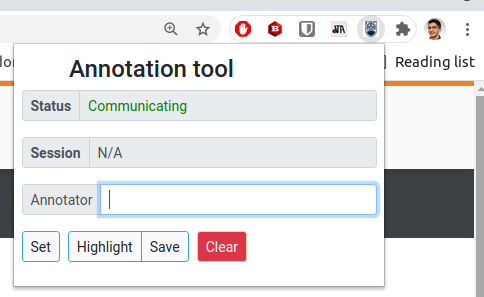
\includegraphics[width=\textwidth]{cp4/annotation-tool}
    \caption{Annotation tool and relevant sentences marked by an annotator}
    \label{fig:corpus-annotation-tool}
\end{figure}




\subsection{Results}


Annotation required a total of \red{$\approx60$} hours of manual work and it was done throughout the course of 4 weeks.
On average the text deemed useful to a software task in the annotated artifacts comprises 
\red{5} sentences. 
Table~\ref{tbl:corpus-annotation-summary} provides summary statistics for the text marked by 
the annotators over all the artifacts inspected as well as on an artifact type basis.


\begin{table}[H]
\centering    
\caption{Summary statistics for the text deemed useful by annotators across the artifacts inspected in the \acs{DS-android} corpus}
\label{tbl:corpus-annotation-summary}
\begin{scriptsize}
\begin{threeparttable}
\begin{tabular}{lcccccc}





& \multicolumn{3}{c}{\textbf{\# of sentences marked}}
& \multicolumn{3}{c}{\textbf{\% of sentences marked by}}
\\ \cmidrule(l){2-4} \cmidrule(l){5-7} 
& total & mean & stdv 
& 1 annot. & 2 annot. & 3 annot. \\

\hline

\textbf{API documentation} 
& 327 & 9.62 & 7.88
& 76\% & 16\% & 7\%
\\
\textbf{GitHub issues} 
& 146 & 4.87 & 3.37
& 74\% & 20\% & 6\%
\\
\textbf{SO answers} 
& 330 & 7.33 & 5.08
& 57\% & 22\% & 21\%
\\
\textbf{Miscellaneous Web pages} 
& 590 & 12.55 & 9.88
& 75\% & 17\% & 8\%
\\

\hline
\textbf{Overall} 
& 1393 & 8.93 & 7.78
& 71\% & 19\% & 10\%
\\
\hline

\end{tabular}
\begin{tablenotes}
    \item[annot] annotator(s);
\end{tablenotes}
\end{threeparttable}
\end{scriptsize}
\end{table}





To that end, we use Nenkova and Passonneau's
pyramid method~\cite{Nenkova2004}. This method was originally used
to quantify the content of summaries produced by different annotators.
The more annotators who include the same content in their summaries,
the more consistent the view of information relevant to a summary and
the more weight given the selected content. We apply the same rationale
to assess the level of agreement of which HUs are relevant to a task
and whether agreement relates to how correctly
a participant completes a task.




To construct the pyramid, we assign a weight to each HU
corresponding to the number of participants who highlighted that HU during
a task.
Figure~\ref{fig:highlights-distribution} shows the distribution of these weights.
From the 602 HUs, we observe that 18\% of them are considered relevant by eight or more participants while 58\% are relevant to only one or two participants.





% Since individuals might use different criteria to
% assess relevance~\cite{Barry1994, Barry1998, Freund2015},
% there is a risk that
% the text selected by annotators does not overlap~\cite{Freund2013, Freund2015}.
% Due to this reason, golden data in \acs{DS-android-small} consists of any sentence marked by annotators. 

% Section~\ref{cp4:threats} further details threats that might arise from this decision.



% Additionally, the text selected by a single annotator may still be crucial for task completion~\cite{marques2020}.


\subsubsection{Metrics}

To compute an approach's accuracy, we use standard \textit{precision} and \textit{recall} metrics~\cite{Manning2009IR} and the text marked by the human annotators in \acs{DS-android-small}.
Since the text marked by them varies, we compute metrics when the manually produced golden data consists of the text marked by one, two, or the three annotators (i.e., $n=1, 2,$ or $3$).

\gm{I am not quite following ratio here...}
\art{I removed references to ratio and started using accuracy}



To ease interpreting precision and recall, Table~\ref{tbl:type-I-II-errors} show all possible evaluation outcomes. The \textit{relevant} and \textit{not-relevant} columns represent the text 
marked (or not) by the annotators. Rows represent the text automatically identified by an automatic approach.


\begin{table}[H]
\centering    
\begin{scriptsize}
\begin{threeparttable}
\begin{tabular}{l|l|l}

\hline

\textbf{}
& \textbf{Relevant}    
& \textbf{Not-relevant} \\

\hline
\hline

\textbf{Identified as relevant} & true positive ($TP$) & false positive ($FP$) \\
\hline
\textbf{Identified as Not-relevant} & false negative ($FN$) & true negative ($TN$) \\
\hline

\end{tabular}
\end{threeparttable}
\end{scriptsize}
\caption{Result outcomes}
\label{tbl:type-I-II-errors}
\end{table}

    



For a given task $t$ and artifact $a$, $precision_n$ is the fraction of the sentences identified that are marked as relevant by $n$ annotators over the total number of sentences identified, as shown in Equation~\ref{eq:cp4:precision}. For example, \textit{precision(t, API documentation)\textsubscript{2}} computes the number of sentences identified by \acs{Krec} for the task $t$ when 
golden data consist of sentences marked by two or more annotators.


\begin{equation}
\label{eq:cp4:precision}    
    Precision(t, a)_n = \frac{TP}{TP + FP}
\end{equation}


Recall ($recall_n$) represents how many of all sentences marked by at least $n$ annotators are identified by a technique (Equation~\ref{eq:cp4:recall}).


\begin{equation}
\label{eq:cp4:recall}        
    Recall(t, a)_n = \frac{TP}{TP + FN}
\end{equation}

% \vspace{3mm}




% \subsection{Results}
% \textcolor{white}{force ident} % this is just for the chapter outline


% --- Discuss results.\footnote{\red{think which summary tables should I have in the thesis body and which I can move to Appendices}} \vspace{3mm}



% --- Precision~\ref{tbl:ds-small-results-precision}  \vspace{3mm}


% --- Recall~\ref{tbl:ds-small-results-recall} \vspace{3mm}

% --- Likely explanation for the results obtained.

% % When interpreting results, we favor precision instead of recall.
% % A false positives may contribute to a developer abandoning reading of an artifact that would otherwise provide crucial information for her task~\cite{Rastkar2010}.




% \begin{table}[H]
\centering    
\begin{scriptsize}
\begin{threeparttable}
\begin{tabular}{lcccccc}

\hline


\multirow{2.5}{*}{Technique}
& \multicolumn{2}{c}{\textit{$Precision_{n=3}$}}
& \multicolumn{2}{c}{\textit{$Precision_{n=2}$}}
& \multicolumn{2}{c}{\textit{$Precision_{n=1}$}}
\\ \cmidrule(l){2-3} \cmidrule(l){4-5} \cmidrule(l){6-7} 


& \textit{mean}
& \textit{std}
& \textit{mean}
& \textit{std}
& \textit{mean}
& \textit{std}
\\


\hline
\hline

\acs{AnsBot} 
& 0.5 & 0.5 % = 3
& 0.5 & 0.5 % = 2
& 0.5 & 0.5 % = 1
\\

\acs{Krec} 
& 0.5 & 0.5 % = 3
& 0.5 & 0.5 % = 2
& 0.5 & 0.5 % = 1
\\

\acs{Hurried} 
& 0.5 & 0.5 % = 3
& 0.5 & 0.5 % = 2
& 0.5 & 0.5 % = 1
\\

\hline

\end{tabular}
\end{threeparttable}
\end{scriptsize}
\caption{Precision of each technique for the tasks of \acs{DS-android-small}}
\label{tbl:ds-small-results-precision}
\end{table}

    

% \begin{table}[H]
% \centering    
% \begin{scriptsize}
% \begin{threeparttable}
% \begin{tabular}{lcccccccccccc}

% \hline


% \multirow{2.5}{*}{Technique}
% & \multicolumn{10}{c}{\textit{Tasks}} 
% & \multicolumn{2}{c}{\textit{Precision}}
% \\  \cmidrule(l){2-11} \cmidrule(l){12-13} 



% &
% \textit{T1} & \textit{T2} & \textit{T3} & \textit{T4} & \textit{T5}
% & \textit{T6} & \textit{T7} & \textit{T8} & \textit{T9} & \textit{T10}
% & \textit{mean}
% & \textit{std}
% \\


% \hline
% \hline

% \acs{AnsBot} 
% & 0.5 & 0.5 & 0.5 & 0.5 & 0.5
% & 0.5 & 0.5 & 0.5 & 0.5 & 0.5
% & 0.5 % mean
% & 0.5 % std
% \\

% \acs{Krec} 
% & 0.5 & 0.5 & 0.5 & 0.5 & 0.5
% & 0.5 & 0.5 & 0.5 & 0.5 & 0.5
% & 0.5 % mean
% & 0.5 % std
% \\

% \acs{Hurried} 
% & 0.5 & 0.5 & 0.5 & 0.5 & 0.5
% & 0.5 & 0.5 & 0.5 & 0.5 & 0.5
% & 0.5 % mean
% & 0.5 % std
% \\

% \hline

% \end{tabular}
% \end{threeparttable}
% \end{scriptsize}
% \caption{Precision of each technique for the tasks of \acs{DS-android-small}}
% \label{tbl:ds-small-results-precision}
% \end{table}

    

% \begin{table}[H]
\centering    
\begin{scriptsize}
\begin{threeparttable}
\begin{tabular}{lcccccc}

\hline


\multirow{2.5}{*}{Technique}
& \multicolumn{2}{c}{\textit{$Recall_{n=3}$}}
& \multicolumn{2}{c}{\textit{$Recall_{n=2}$}}
& \multicolumn{2}{c}{\textit{$Recall_{n=1}$}}
\\ \cmidrule(l){2-3} \cmidrule(l){4-5} \cmidrule(l){6-7} 


& \textit{mean}
& \textit{std}
& \textit{mean}
& \textit{std}
& \textit{mean}
& \textit{std}
\\


\hline
\hline

\acs{AnsBot} 
& 0.5 & 0.5 % = 3
& 0.5 & 0.5 % = 2
& 0.5 & 0.5 % = 1
\\

\acs{Krec} 
& 0.5 & 0.5 % = 3
& 0.5 & 0.5 % = 2
& 0.5 & 0.5 % = 1
\\

\acs{Hurried} 
& 0.5 & 0.5 % = 3
& 0.5 & 0.5 % = 2
& 0.5 & 0.5 % = 1
\\

\hline

\end{tabular}
\end{threeparttable}
\end{scriptsize}
\caption{Recall of each technique for the tasks of \acs{DS-android-small}}
\label{tbl:ds-small-results-recall}
\end{table}

    


% \subsection{Threats}
% \label{cp4:corpus-threats}

% --- \red{Argue that this is not a replication study but rather establishing thresholds} \vspace{3mm}

% --- Discuss threats \vspace{3mm}



